\documentclass[10pt,letterpaper]{article}

% ---------------------------------------------------------------------------
% SuSchedule-r final report (LaTeX source)
% Compile with: pdflatex CS455_SuSchedule-r_Report.tex
% ---------------------------------------------------------------------------

\usepackage[margin=0.72in]{geometry}
\usepackage[T1]{fontenc}
\usepackage[utf8]{inputenc}
\usepackage{lmodern}
\usepackage{microtype}
\usepackage{xcolor}
\usepackage{booktabs}
\usepackage{tabularx}
\usepackage{array}
\usepackage{enumitem}
\usepackage{titlesec}
\usepackage{fancyhdr}
\usepackage{hyperref}
\usepackage{tcolorbox}
\usepackage{listings}
\usepackage{amsmath}
\usepackage{amssymb}
\usepackage{graphicx}
\usepackage{tikz}
\usetikzlibrary{arrows.meta,positioning,fit,backgrounds,shapes.geometric,calc}

\definecolor{suNavy}{HTML}{002776}
\definecolor{suBlue}{HTML}{1C47A8}
\definecolor{suLight}{HTML}{EEF3FF}
\definecolor{suLine}{HTML}{C9D2E5}
\definecolor{suText}{HTML}{182033}
\definecolor{suMuted}{HTML}{5C657F}
\definecolor{suWarn}{HTML}{8A4B00}

\hypersetup{
  colorlinks=true,
  linkcolor=suBlue,
  urlcolor=suBlue,
  citecolor=suBlue,
  pdftitle={SuSchedule-r Final Report},
  pdfauthor={Kerem Sirtikizil, Cagan Cakir, Eray Cagan Ozdemir}
}

\pagestyle{fancy}
\fancyhf{}
\lhead{\textcolor{suMuted}{SuSchedule-r}}
\rhead{\textcolor{suMuted}{CS 455 Final Project}}
\cfoot{\thepage}
\renewcommand{\headrulewidth}{0.4pt}
\renewcommand{\headrule}{\hbox to\headwidth{\color{suLine}\leaders\hrule height \headrulewidth\hfill}}

\titleformat{\section}
  {\large\bfseries\color{suNavy}}
  {\thesection}{0.6em}{}
  [\vspace{-0.35em}\color{suLine}\titlerule]
\titleformat{\subsection}
  {\normalsize\bfseries\color{suBlue}}
  {\thesubsection}{0.6em}{}
\titleformat{\subsubsection}
  {\normalsize\bfseries\color{suText}}
  {\thesubsubsection}{0.6em}{}

\setlength{\parindent}{0pt}
\setlength{\parskip}{4pt}
\setlist[itemize]{leftmargin=1.2em,itemsep=2pt,topsep=2pt}
\setlist[enumerate]{leftmargin=1.4em,itemsep=2pt,topsep=2pt}
\renewcommand{\arraystretch}{1.12}

\newcolumntype{Y}{>{\raggedright\arraybackslash}X}
\newcommand{\code}[1]{\texttt{#1}}
\newcommand{\yes}{\(\checkmark\)}
\newcommand{\no}{\(\times\)}

\lstdefinestyle{codeblock}{
  basicstyle=\ttfamily\footnotesize,
  breaklines=true,
  frame=single,
  rulecolor=\color{suLine},
  backgroundcolor=\color{suLight},
  columns=fullflexible,
  keepspaces=true,
  showstringspaces=false
}
\lstset{style=codeblock}

\newtcolorbox{summarybox}{
  colback=suLight,
  colframe=suNavy,
  boxrule=0.7pt,
  arc=2pt,
  left=7pt,
  right=7pt,
  top=6pt,
  bottom=6pt
}

\newtcolorbox{findingbox}{
  colback=white,
  colframe=suLine,
  boxrule=0.6pt,
  arc=2pt,
  left=7pt,
  right=7pt,
  top=6pt,
  bottom=6pt
}

\tikzset{
  archBox/.style={
    draw=suLine,
    rounded corners=3pt,
    fill=white,
    line width=0.55pt,
    align=center,
    font=\sffamily\small,
    minimum height=9mm,
    text width=33mm
  },
  archBlue/.style={
    archBox,
    draw=suBlue,
    fill=suLight
  },
  archNavy/.style={
    archBox,
    draw=suNavy,
    fill=suNavy!7
  },
  archData/.style={
    archBox,
    fill=suLine!23,
    text width=30mm
  },
  archDecision/.style={
    diamond,
    draw=suBlue,
    fill=suLight,
    aspect=2.1,
    align=center,
    font=\sffamily\small,
    inner sep=1.5pt
  },
  archArrow/.style={
    -{Latex[length=2.5mm]},
    line width=0.65pt,
    draw=suBlue
  },
  archMutedArrow/.style={
    -{Latex[length=2.2mm]},
    line width=0.55pt,
    draw=suMuted,
    dashed
  },
  archGroup/.style={
    draw=suLine,
    rounded corners=4pt,
    fill=suLight!30,
    inner sep=5pt
  },
  numCircle/.style={
    circle,
    draw=suNavy,
    fill=suNavy,
    text=white,
    font=\sffamily\bfseries\scriptsize,
    minimum size=5.2mm,
    inner sep=0pt
  }
}

\begin{document}

\begin{center}
  {\Huge\bfseries\color{suNavy} SuSchedule-r}\\[4pt]
  {\Large A Retrieval-Augmented, Tool-Using Course-Planning Agent}\\[-1pt]
  {\Large for Sabanci University}\\[10pt]
  {\bfseries CS 455 / CS 555 -- Large Language Models}\\
  Final Project Report \(\cdot\) Sabanci University\\[8pt]
  \textbf{Track:} CS 455 Project\\[4pt]
  Kerem Sirtikizil (32298) \quad
  Cagan Cakir (32254) \quad
  Eray Cagan Ozdemir (32136)
\end{center}

\begin{summarybox}
\textbf{Abstract.}
SuSchedule-r is a course-advising assistant that grounds a large-language-model agent in Sabanci University's real course catalogue, prerequisite graph, degree requirements, and weekly section offerings. The system combines a FAISS-backed two-stage semantic retriever (BGE bi-encoder plus optional cross-encoder re-ranker over \textbf{817 courses}) with a GPT-4o \textbf{ReAct} tool-calling agent and an interactive web UI whose schedule builder renders a weekly calendar with live conflict detection.

We evaluate the system on four axes with labeled, reproducible test sets: retrieval quality, time-conflict detection, degree-requirement accuracy, and end-to-end answer grounding. The bi-encoder retriever reaches \textbf{Hit@5 = 0.977} and \textbf{Recall@10 = 0.966}; the conflict checker is \textbf{100\% accurate} on labeled meeting pairs and returns \textbf{0 unsound schedules} over corequisite-expanded real course bundles; and the ReAct agent grounds \textbf{11/12} end-to-end answers, with the single failure isolated to a provisional open-ended recommendation label. We report negative results honestly: the cross-encoder re-ranker hurts short topical retrieval metrics, the graph requirement engine over-counts remaining required credits by \textbf{4 SU} because it lacks a course-substitution table, future-term schedules use a proxy offering term until the registrar publishes the target term, and the ReAct agent can still be inconsistent when it emits slightly malformed tool parameters.
\end{summarybox}

\section{Introduction}

\subsection{Problem}
Each semester, a Sabanci student needs to choose courses while balancing degree requirements, prerequisites, credit limits, and weekly meeting conflicts. The decision is not just a search problem. A course may be relevant to a student's interests but unavailable, ineligible because of prerequisites, outside the student's degree requirement pool, or impossible to fit into an existing schedule because of a lecture, lab, or recitation conflict.

General-purpose LLMs are fluent but unreliable in this domain. They can invent course codes, confuse course titles, miss recitations, or ignore a student's actual degree audit. For an advising assistant to be useful, factual claims must come from data-backed tools rather than from model memory.

\subsection{Design Principle}
Our design principle is:

\begin{center}
\textbf{Use the LLM for language, intent, explanation, and tool orchestration; use deterministic code for factual constraints.}
\end{center}

The ReAct agent can decide whether to search, inspect a requirement graph, check prerequisites, or validate a schedule. However, the final facts come from deterministic parsers and tools:
\begin{itemize}
  \item course metadata from scraped Sabanci catalogue pages,
  \item prerequisite/corequisite expressions parsed into boolean trees,
  \item per-degree and per-cohort requirement graphs,
  \item Degree Evaluation parsing for the student's official audit,
  \item FAISS retrieval over course descriptions,
  \item timetable conflict detection over normalized meeting intervals.
\end{itemize}

\subsection{Contributions}
\begin{enumerate}
  \item A grounded course-advising system for Sabanci University that combines RAG, graph-based requirements, transcript/degree-evaluation context, and timetable reasoning.
  \item A GPT-4o ReAct agent with a 22-tool toolbox for retrieval, requirements, eligibility, minors, science/engineering credits, timetable construction, and current-schedule checking.
  \item A deterministic data layer: scrapers, prerequisite parser, degree graph builder, offering parser, requirement evaluator, and schedule conflict engine.
  \item A reproducible evaluation suite with human-labeled retrieval and agent datasets, local deterministic tests, live agent tests, ablations, and honest error analysis.
\end{enumerate}

\section{Data and Knowledge Base}

All university knowledge is derived from public Sabanci catalogue/registration pages and the student's own uploaded academic records or Degree Evaluation export.

\begin{table}[h]
\centering
\small
\begin{tabularx}{\linewidth}{@{}p{0.23\linewidth}Yp{0.24\linewidth}@{}}
\toprule
\textbf{Asset} & \textbf{Contents} & \textbf{Current scale} \\
\midrule
Course catalogue & Code, title, description, SU credit, ECTS, prerequisites, corequisites, degree sections, seasons & \textbf{817 courses} \\
Active RAG metadata & One row per indexed course & \textbf{817 rows} \\
FAISS index & BGE-base course embeddings & \textbf{817 x 768} vectors \\
Full prerequisite graph & Parsed prerequisite dependencies & \textbf{721 nodes, 729 edges} \\
Degree/cohort graphs & Per-program, per-admit-year requirement slices & \textbf{14 programs x 5 cohorts x 4 sections} \\
Degree graph files & JSON + gpickle requirement graphs & \textbf{268 JSON, 268 gpickle} \\
Offerings & Section meetings, CRNs, labs, recitations & Terms \textbf{202401--202503} \\
Student audit & Official Banner Degree Evaluation / transcript-derived profile & BSCS-DM sample \\
\bottomrule
\end{tabularx}
\caption{Data assets used by the assistant.}
\end{table}

\subsection{Scraping and Preprocessing}
The scraper pipeline is deterministic and cache-backed. It discovers degree pages, course pools, and course-detail pages; parses course metadata; builds prerequisite graphs; and stores outputs under \code{data/}, \code{courses/}, \code{degrees/}, \code{pools/}, and \code{offerings/}.

The prerequisite parser is a recursive-descent parser. It preserves \code{AND}, \code{OR}, parentheses, minimum grades, and concurrent/corequisite conditions as a boolean expression tree. That tree is stored on graph nodes and evaluated later by the eligibility engine. This matters because expressions such as:

\begin{lstlisting}
(MATH 204 and CS 300) or instructor consent
\end{lstlisting}

cannot be represented safely as a flat list of required courses.

\begin{findingbox}
\textbf{Parser validation.} The prerequisite parser reaches 100\% strict parse coverage on 426 strict expressions, with 0 parser failures. The full graph is acyclic, and external prerequisites are preserved as helper nodes where needed.
\end{findingbox}

\subsection{Requirement Graphs}
Normal planning does \emph{not} use the whole graph. The agent selects scoped graphs from:

\begin{lstlisting}
data/degree_graphs/{PROGRAM}/{COHORT}/{SECTION}.gpickle
data/degree_graphs/{PROGRAM}/{COHORT}/{SECTION}.json
\end{lstlisting}

For example:

\begin{lstlisting}
data/degree_graphs/BSCS-DM/202201/Required.gpickle
data/degree_graphs/BSCS-DM/202201/Core_Elective.gpickle
data/degree_graphs/BSCS-DM/202201/Area_Elective.gpickle
data/degree_graphs/BSCS-DM/202201/Free_Elective.gpickle
\end{lstlisting}

This keeps retrieval and requirement reasoning efficient. Nodes with \code{in\_slice=True} are actual members of the selected requirement/elective pool. Upstream prerequisite-only nodes are retained only as validation helpers.

\section{System Architecture}

\begin{figure}[h]
\centering
\resizebox{\linewidth}{!}{%
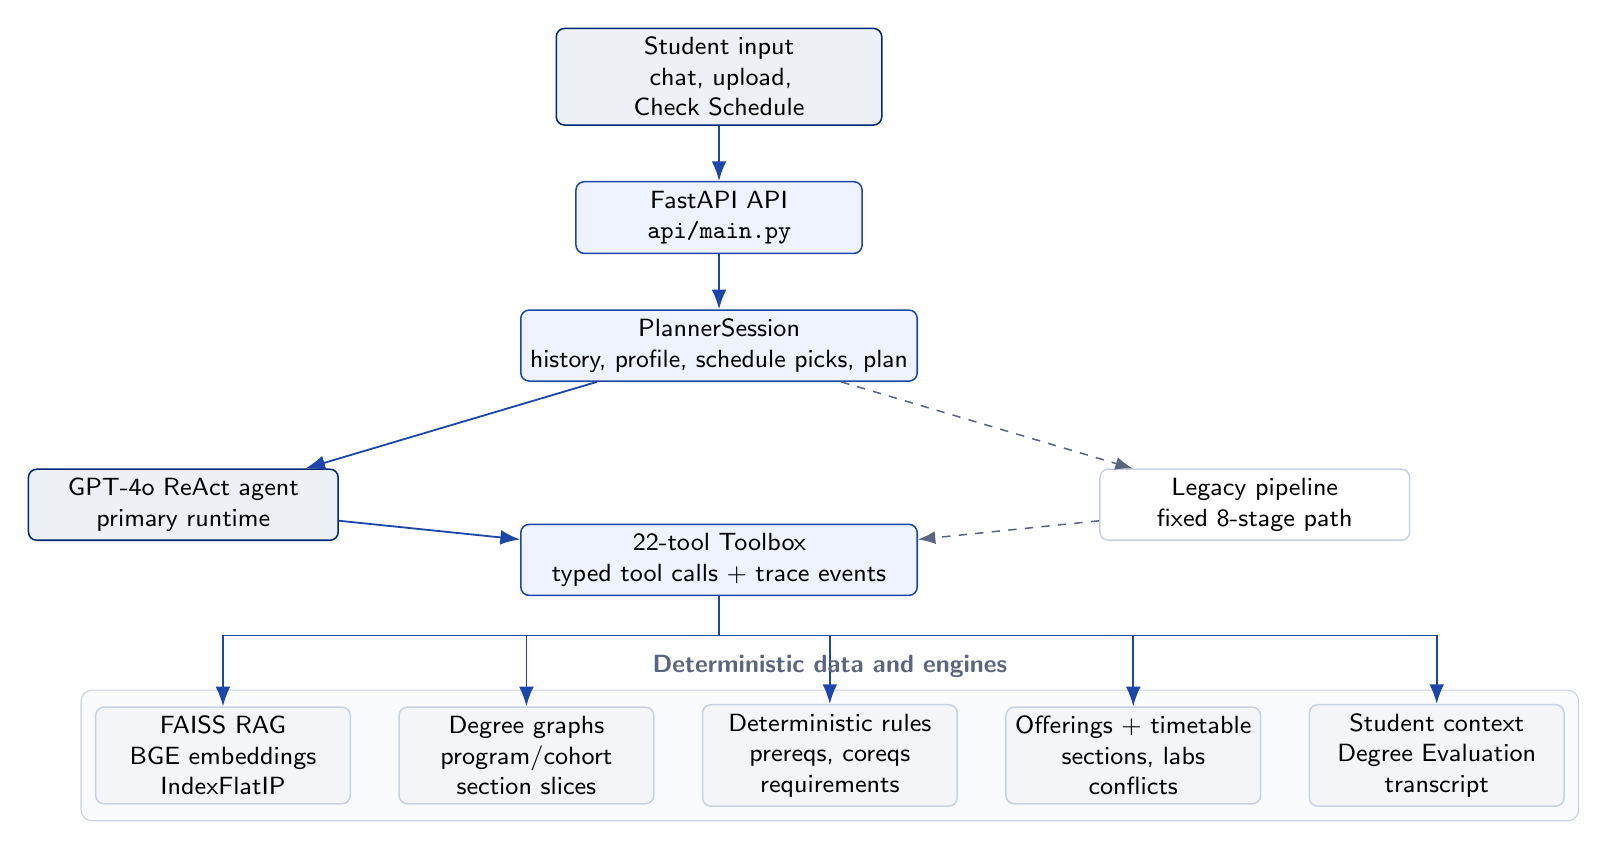
\begin{tikzpicture}[node distance=7mm and 9mm]
  \node[archNavy, text width=39mm] (user) {Student input\\chat, upload, Check Schedule};
  \node[archBlue, below=of user, text width=34mm] (api) {FastAPI API\\\code{api/main.py}};
  \node[archBlue, below=of api, text width=48mm] (session) {PlannerSession\\history, profile, schedule picks, plan};

  \node[archNavy, below left=11mm and 23mm of session, text width=37mm] (react) {GPT-4o ReAct agent\\primary runtime};
  \node[archBox, below right=11mm and 23mm of session, text width=37mm] (pipeline) {Legacy pipeline\\fixed 8-stage path};
  \node[archBlue, below=18mm of session, text width=48mm] (tools) {22-tool Toolbox\\typed tool calls + trace events};

  \node[archData, below=14mm of tools, xshift=-63mm] (faiss) {FAISS RAG\\BGE embeddings\\IndexFlatIP};
  \node[archData, right=6mm of faiss] (graphs) {Degree graphs\\program/cohort\\section slices};
  \node[archData, right=6mm of graphs] (rules) {Deterministic rules\\prereqs, coreqs\\requirements};
  \node[archData, right=6mm of rules] (time) {Offerings + timetable\\sections, labs\\conflicts};
  \node[archData, right=6mm of time] (audit) {Student context\\Degree Evaluation\\transcript};

  \draw[archArrow] (user) -- (api);
  \draw[archArrow] (api) -- (session);
  \draw[archArrow] (session) -- (react);
  \draw[archMutedArrow] (session) -- (pipeline);
  \draw[archArrow] (react) -- (tools);
  \draw[archMutedArrow] (pipeline) -- (tools);

  \foreach \n in {faiss,graphs,rules,time,audit} {
    \draw[archArrow] (tools.south) -- ++(0,-5mm) -| (\n.north);
  }

  \begin{scope}[on background layer]
    \node[archGroup, fit=(faiss)(graphs)(rules)(time)(audit)] (dataGroup) {};
  \end{scope}
  \node[font=\sffamily\bfseries\small, color=suMuted]
    at ($(dataGroup.north)+(0,3mm)$) {Deterministic data and engines};
\end{tikzpicture}}
\caption{SuSchedule-r runtime topology. The LLM chooses actions, but factual constraints are owned by deterministic tools and data stores.}
\end{figure}

\begin{figure}[h]
\centering
\resizebox{0.98\linewidth}{!}{%
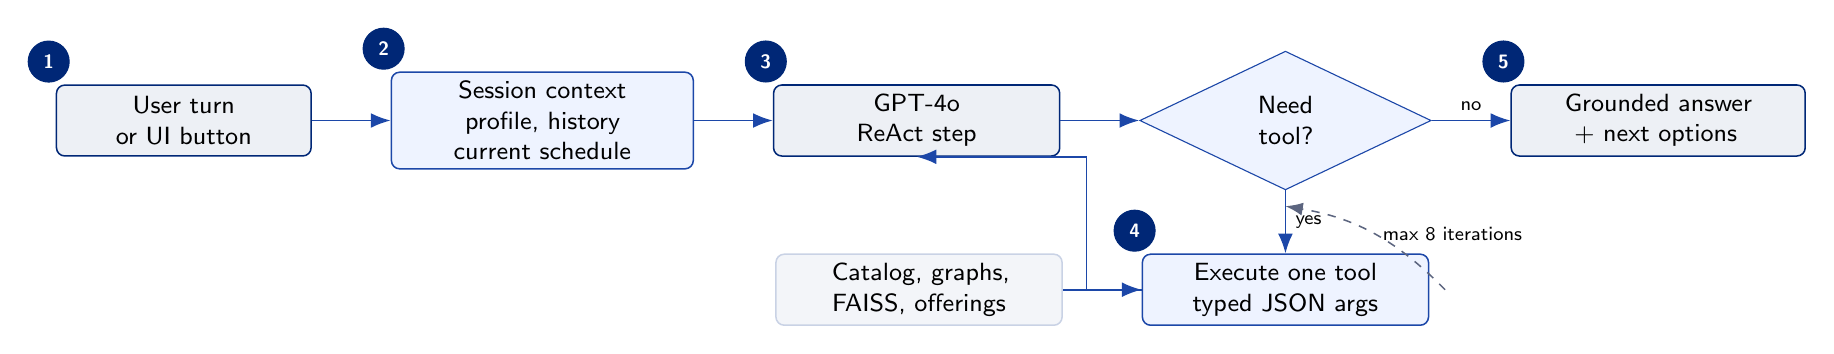
\begin{tikzpicture}[node distance=8mm and 10mm]
  \node[archNavy, text width=30mm] (turn) {User turn\\or UI button};
  \node[archBlue, right=of turn, text width=36mm] (context) {Session context\\profile, history\\current schedule};
  \node[archNavy, right=of context, text width=34mm] (llm) {GPT-4o\\ReAct step};
  \node[archDecision, right=of llm, text width=21mm] (decision) {Need\\tool?};
  \node[archBlue, below=of decision, text width=34mm] (tool) {Execute one tool\\typed JSON args};
  \node[archData, left=of tool, text width=34mm] (facts) {Catalog, graphs,\\FAISS, offerings};
  \node[archNavy, right=of decision, text width=35mm] (answer) {Grounded answer\\+ next options};

  \draw[archArrow] (turn) -- (context);
  \draw[archArrow] (context) -- (llm);
  \draw[archArrow] (llm) -- (decision);
  \draw[archArrow] (decision) -- node[above, font=\scriptsize\sffamily] {no} (answer);
  \draw[archArrow] (decision) -- node[right, font=\scriptsize\sffamily] {yes} (tool);
  \draw[archArrow] (facts) -- (tool);
  \draw[archArrow] (tool.west) -- ++(-7mm,0) |- (llm.south);
  \draw[archMutedArrow] ($(tool.east)+(2mm,0)$) to[bend right=18] node[right, font=\scriptsize\sffamily] {max 8 iterations} ($(decision.south)+(0,-2mm)$);

  \node[numCircle, above left=1mm and -1mm of turn.north west] {1};
  \node[numCircle, above left=1mm and -1mm of context.north west] {2};
  \node[numCircle, above left=1mm and -1mm of llm.north west] {3};
  \node[numCircle, above left=1mm and -1mm of tool.north west] {4};
  \node[numCircle, above left=1mm and -1mm of answer.north west] {5};
\end{tikzpicture}}
\caption{One ReAct turn. Tool results are appended to the model context; high-impact actions such as \code{set\_plan()} remain guarded by deterministic validation.}
\end{figure}

\begin{figure}[h]
\centering
\resizebox{\linewidth}{!}{%
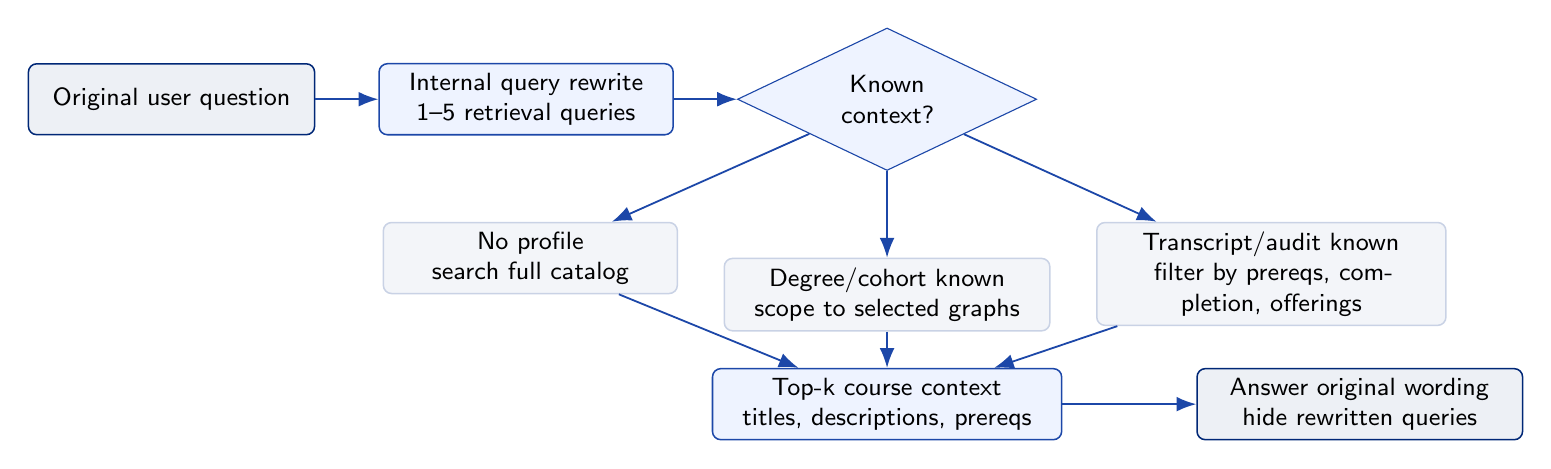
\begin{tikzpicture}[node distance=8mm and 8mm]
  \node[archNavy, text width=34mm] (q) {Original user question};
  \node[archBlue, right=of q, text width=35mm] (rewrite) {Internal query rewrite\\1--5 retrieval queries};
  \node[archDecision, right=of rewrite, text width=22mm] (profile) {Known\\context?};

  \node[archData, below left=11mm and 17mm of profile, text width=35mm] (full) {No profile\\search full catalog};
  \node[archData, below=11mm of profile, text width=39mm] (degree) {Degree/cohort known\\scope to selected graphs};
  \node[archData, below right=11mm and 17mm of profile, text width=42mm] (eligible) {Transcript/audit known\\filter by prereqs, completion, offerings};

  \node[archBlue, below=25mm of profile, text width=42mm] (topk) {Top-k course context\\titles, descriptions, prereqs};
  \node[archNavy, right=17mm of topk, text width=39mm] (final) {Answer original wording\\hide rewritten queries};

  \draw[archArrow] (q) -- (rewrite);
  \draw[archArrow] (rewrite) -- (profile);
  \draw[archArrow] (profile) -- (full);
  \draw[archArrow] (profile) -- (degree);
  \draw[archArrow] (profile) -- (eligible);
  \draw[archArrow] (full) -- (topk);
  \draw[archArrow] (degree) -- (topk);
  \draw[archArrow] (eligible) -- (topk);
  \draw[archArrow] (topk) -- (final);
\end{tikzpicture}}
\caption{Scoped RAG behavior. The system avoids searching the whole graph during degree-specific planning and uses full-catalog FAISS only for exploratory questions.}
\end{figure}

\subsection{RAG Pipeline}
The RAG pipeline has two stages:
\begin{enumerate}
  \item \textbf{Bi-encoder first stage.} \code{BAAI/bge-base-en-v1.5} encodes the query and searches \code{embeddings/su\_courses.index}, a FAISS \code{IndexFlatIP} index over L2-normalized vectors.
  \item \textbf{Cross-encoder re-ranking.} \code{BAAI/bge-reranker-base} can re-rank the first-stage candidates.
\end{enumerate}

FAISS is mandatory. If the FAISS index is missing or inconsistent with the metadata/embedding matrix, the retriever raises an error instead of silently switching to a NumPy search backend. Filtered retrieval uses FAISS \code{IDSelectorBatch}, so degree, section, subject, and eligible-course scopes are enforced inside the vector search.

\subsection{ReAct Agent}
The primary runtime mode is a single \textbf{tool-calling ReAct agent}, not a multi-agent system. GPT-4o receives a stable system prompt, recent chat history, structured student context, and 22 available tools. It can call tools for factual information and then produce a final answer.

The loop is capped at \textbf{8 iterations} per turn. Conversation history is capped by turn count, while structured student state is kept outside history so it survives trimming. The model is proactive through options, but \code{set\_plan()} is only allowed after the user explicitly asks to create or commit a plan.

\subsection{Deterministic Guardrails}
The LLM is not trusted to validate hard constraints:
\begin{itemize}
  \item \code{eligibility.py} evaluates prerequisite/corequisite boolean trees.
  \item \code{requirements.py} computes remaining required/core/area/free courses.
  \item \code{degree\_eval.py} parses official Degree Evaluation HTML.
  \item \code{timetable.py} detects time overlaps and searches feasible section combinations.
  \item \code{react\_agent.py} repairs unsupported course titles and schedule claims using tool traces.
  \item \code{set\_plan()} refuses to commit an invalid plan.
\end{itemize}

\subsection{Web UI}
The FastAPI + vanilla JavaScript UI has chat, trace visibility, file upload, a schedule builder with real course sections, lab/recitation rows through corequisite expansion, weekly calendar rendering, current-schedule conflict checking, and a ``Check Schedule'' agent review grounded in server-computed conflicts.

Because Fall 2026 (\code{202601}) does not have real published offerings yet, scheduling uses the most recent same-season proxy term (\code{202501}) and labels this clearly.

\section{Evaluation Methodology}

The project announcement asks for a working system, appropriate metrics, honest error analysis, reproducibility, and a clear README. We evaluate four components using version-controlled datasets in \code{eval/}.

\begin{table}[h]
\centering
\small
\begin{tabularx}{\linewidth}{@{}p{0.29\linewidth}Yp{0.17\linewidth}@{}}
\toprule
\textbf{Runner} & \textbf{Measures} & \textbf{OpenAI?} \\
\midrule
\code{eval.run\_retrieval} & Hit@k, Recall@k, MRR@10, nDCG@10, re-ranker ablation, FAISS backend evidence & No \\
\code{eval.run\_conflicts} & Interval-overlap accuracy, corequisite-expanded timetable soundness and feasibility & No \\
\code{eval.run\_requirements} & Official Degree Evaluation credit gaps vs graph engine & No \\
\code{eval.run\_agent} & Answer grounding, required tool/action success, task success, latency, token cost & Yes \\
\code{eval.run\_agent --dataset general...} & Transcript-free catalog chat, RAG behavior, Check Schedule behavior, and forbidden planning actions & Yes \\
\code{eval.run\_agent --rescore} & Re-score saved raw agent answers after label edits & No \\
\bottomrule
\end{tabularx}
\caption{Evaluation runners.}
\end{table}

\subsection{Human-Labeled Tests}
\code{eval/retrieval\_queries.json} contains \textbf{44 natural-language queries} with gold course codes. Labels are high-precision rather than exhaustive. The dataset includes \textbf{34 existing} reviewed labels and \textbf{10 provisional} exploratory labels.

\code{eval/agent\_questions.json} contains \textbf{13 conversation questions} with structured checks: required course codes, forbidden course codes, required terms, credit facts, regex patterns, required semantic actions, and forbidden actions. The final row preloads UI schedule-builder picks and tests the \textbf{Check Schedule} button path: the agent must call \code{get\_current\_schedule} rather than inventing a new timetable. One ambiguous recommendation case is marked provisional.

\code{eval/general\_conversation\_questions.json} contains \textbf{9 transcript-free conversation questions}. These test normal course chat before a transcript is uploaded: RAG-backed recommendations, single-course explanations, permission-respecting planning behavior, direct timetable checks, and a transcript-free Check Schedule scenario that must avoid degree-progress claims.

\textbf{Profile diversity and privacy.} We originally planned to evaluate more real student profiles. In practice, profile diversity stayed low because official Degree Evaluation files contain almost a student's entire academic life: completed courses, failed/withdrawn attempts, transfer credits, GPA-related progress, degree status, and remaining graduation requirements. Several students were not comfortable disclosing that information, even for a course project. Therefore, the current live profile-backed evaluation focuses on one consented BSCS-DM profile, while the data layer itself covers 14 programs, 5 cohorts, and transcript-free general conversation scenarios.

\subsection{Representative 20-Case Human Test Matrix}
To make the human evaluation scope explicit, we maintain a 20-case coverage matrix in \code{eval/submission\_human\_cases.json}. It combines runnable benchmark themes with reviewer-facing behavioral checks across retrieval, exact catalog facts, degree reasoning, schedule reasoning, planning permission, and minor/credit-rule tools.

\begin{table}[h]
\centering
\scriptsize
\begin{tabularx}{\linewidth}{@{}p{0.07\linewidth}p{0.18\linewidth}YY@{}}
\toprule
\textbf{ID} & \textbf{Area} & \textbf{User scenario} & \textbf{Human label / expected behavior} \\
\midrule
H01 & Catalog RAG & Learn machine learning & Retrieve CS 412 and/or CS 415; explain from catalog context. \\
H02 & Catalog RAG & Operating systems internals & Retrieve CS 307; explain OS concepts. \\
H03 & Catalog RAG & Database design and querying & Retrieve CS 306; avoid unrelated data-mining answers. \\
H04 & Catalog RAG & Energy and sustainability & Use full-catalog search, not CS-only guesses. \\
H05 & Exact fact & CS 412 SU credits & Call exact lookup; answer 3 SU credits. \\
H06 & Prerequisites & CS 301 prerequisites & Mention CS 300 and MATH 204. \\
H07 & Corequisite & CS 412 recitation & Mention CS 412R and preserve its title. \\
H08 & Course content & CS 445 coverage & Explain NLP / language-processing content smoothly. \\
H09 & General chat & Networking recommendations & Use RAG, suggest relevant networking/security courses, no plan commit. \\
H10 & Focus area & Theoretical CS & Surface theory courses such as algorithms/complexity/formal languages. \\
H11 & Cross-program & IE optimization / OR & Prefer IE/OR courses such as IE 311, IE 312, IE 313. \\
H12 & LLM/NLP interest & LLM and NLP courses & Retrieve CS 445 / CS 412 / CS 415-style options. \\
H13 & Requirements & Loaded degree evaluation & Use profile state; do not ask again for degree/cohort/transcript. \\
H14 & Scoped electives & CS security/networking Core/Area & Select degree/cohort graph and retrieve inside scoped pools. \\
H15 & Planning permission & Plan request without profile & Ask for missing profile; do not call \code{set\_plan}. \\
H16 & Validated planning & Plan next semester with profile & Validate prereqs/credits before committing. \\
H17 & Timetable & CS 412 + CS 302 together & Call \code{build\_timetable}; include recitation conflicts. \\
H18 & UI schedule & Check Schedule button & Call \code{get\_current\_schedule}; keep selected sections fixed. \\
H19 & Candidate fit & Add CS 405 to current schedule & Call \code{check\_courses\_against\_current\_schedule}. \\
H20 & Minor/credits & Finance minor + eng/sci credits & Use minor and Engineering/Basic-Science credit tools. \\
\bottomrule
\end{tabularx}
\caption{Representative 20-sample human-labeled coverage matrix.}
\end{table}

\section{Results}

\subsection{Rule-Based Baselines and Tool Equivalence}
The instructor feedback suggested a traditional rule-based baseline. In our architecture, the deterministic functions themselves are that baseline for hard constraints. For prerequisites, degree requirements, science/engineering credits, and timetable conflicts, the ReAct agent does not invent an answer: it calls the same rule-based functions that can be run without the LLM.

\begin{table}[h]
\centering
\small
\begin{tabularx}{\linewidth}{@{}p{0.27\linewidth}YY@{}}
\toprule
\textbf{Task type} & \textbf{Rule-based component} & \textbf{Relation to ReAct answer} \\
\midrule
Prerequisite/corequisite checks & \code{eligibility.py}, \code{get\_course\_details}, \code{check\_prereqs} & Same factual result; the LLM only explains it in natural language. \\
Degree progress & \code{requirements.py}, \code{degree\_eval.py} & Same remaining-credit/course computation; the LLM formats and contextualizes it. \\
Timetable conflicts & \code{timetable.py}, \code{get\_current\_schedule}, \code{build\_timetable} & Same conflict pairs and feasibility result; the LLM summarizes the schedule. \\
Catalog topic search & FAISS retriever + optional re-ranker & Hybrid benefit: semantic retrieval narrows candidates, then the LLM explains relevance. \\
\bottomrule
\end{tabularx}
\caption{Rule-based baseline interpretation. Hard constraints are already deterministic; ReAct adds orchestration and language rather than replacing the baseline.}
\end{table}

This means the rule-based baseline and function-call results are intentionally identical for factual constraint checks. The meaningful comparison is not whether the LLM can beat the rule engine on rules; it should not try. The comparison is whether the hybrid system can combine those rule outputs with RAG-based semantic course discovery and a smooth conversational interface.

\subsection{Retrieval}
The current retriever uses FAISS \code{IndexFlatIP} with \textbf{817 vectors}. The retrieval evaluation confirms \textbf{88 FAISS searches} and no NumPy search backend.

\begin{table}[h]
\centering
\small
\begin{tabular}{@{}lrrr@{}}
\toprule
\textbf{Metric} & \textbf{Re-ranker ON} & \textbf{Re-ranker OFF} & \textbf{Delta} \\
\midrule
Hit@1 & 0.773 & \textbf{0.909} & -0.136 \\
Hit@5 & 0.955 & \textbf{0.977} & -0.023 \\
Recall@5 & 0.875 & \textbf{0.928} & -0.053 \\
Recall@10 & 0.943 & \textbf{0.966} & -0.023 \\
MRR@10 & 0.859 & \textbf{0.938} & -0.079 \\
nDCG@10 & 0.849 & \textbf{0.922} & -0.073 \\
\bottomrule
\end{tabular}
\caption{Retrieval metrics over 44 labeled queries.}
\end{table}

Recall@10 by review status:

\begin{table}[h]
\centering
\small
\begin{tabular}{@{}lrr@{}}
\toprule
\textbf{Label group} & \textbf{n} & \textbf{Recall@10, re-ranker ON} \\
\midrule
existing & 34 & 0.985 \\
provisional & 10 & 0.800 \\
\bottomrule
\end{tabular}
\end{table}

The bi-encoder alone outperforms the cross-encoder on all six metrics. This is an important negative result: for short topical catalogue queries, exact semantic embedding search is already strong and the cross-encoder sometimes promotes broadly related but less appropriate courses.

\subsection{Conflict Detection and Timetable Soundness}

\begin{table}[h]
\centering
\small
\begin{tabularx}{0.78\linewidth}{@{}Yr@{}}
\toprule
\textbf{Check} & \textbf{Result} \\
\midrule
Labeled meeting pairs & 12 \\
Accuracy / precision / recall & \textbf{1.000 / 1.000 / 1.000} \\
Real course bundles & 6 \\
Unsound schedules returned & \textbf{0} \\
Wrong feasibility classifications & \textbf{0} \\
Missing required lab/recitation picks & \textbf{0} \\
Feasibility accuracy & \textbf{1.000} \\
\bottomrule
\end{tabularx}
\end{table}

The bundle tests start with lecture choices and then auto-add direct catalog corequisites such as \code{CS 412R}, \code{CS 308L}, and \code{MATH 101R}. This directly tests a practical scheduling issue: a lecture-only plan can look conflict-free while its required lab/recitation makes it impossible.

\subsection{Degree Requirements}
The official Banner Degree Evaluation is treated as ground truth for credit completion.

\begin{table}[h]
\centering
\small
\begin{tabular}{@{}lrrr@{}}
\toprule
\textbf{Section} & \textbf{Min SU} & \textbf{Completed SU} & \textbf{Remaining SU} \\
\midrule
University Courses & 41 & 41 & 0 \\
Core Electives & 31 & 31 & 0 \\
Required Courses & 29 & 26 & 3 \\
Area Electives & 9 & 9 & 0 \\
Free Electives & 15 & 15 & 0 \\
General & 125 & 122 & 3 \\
\bottomrule
\end{tabular}
\end{table}

The graph engine reports \code{CS 395}, \code{ENS 492}, and \code{MATH 212} still required, with \textbf{7 SU} required credits left. The discrepancy against the official Required bucket is \textbf{+4 SU}, a conservative over-count caused by missing course-substitution/equivalence logic.

\subsection{End-to-End ReAct Agent}

The saved result below is the latest completed live run over the earlier 12-question agent set. After adding the \code{a13} Check Schedule row and the 9-row general conversation set, the live agent evaluation should be rerun before quoting final updated metrics.

\begin{table}[h]
\centering
\small
\begin{tabularx}{0.75\linewidth}{@{}Yr@{}}
\toprule
\textbf{Metric} & \textbf{Value} \\
\midrule
Questions & 12 \\
Answer grounding accuracy & \textbf{0.917} \\
Action success accuracy & \textbf{1.000} \\
Task success accuracy & \textbf{0.917} \\
Existing-label task success & \textbf{11/11} \\
Provisional-label task success & \textbf{0/1} \\
Average latency & 8.59 s \\
Average tokens & 6,691 \\
Average tool calls & 0.5 \\
\bottomrule
\end{tabularx}
\end{table}

The single failed item is the provisional optimization/operations-research recommendation. The model suggested \code{CS 306} and justified it through database query optimization, but the provisional gold labels expected IE/OR-flavored courses such as \code{IE 311}, \code{IE 312}, or \code{IE 313}. We count this as a real failure in the reported 12-question score, while also flagging that the accepted answer set for this broad recommendation needs human review.

\subsection{API Cost and Context Controls}
The current ReAct implementation is intentionally not fully token-optimized. In the measured live run, the average answer used about \textbf{6.7k tokens}. With GPT-4o pricing, a typical non-optimized tool-calling message is roughly on the order of \textbf{two US cents}, depending on the prompt/completion split and number of tool calls.

The cost risk is context growth. Each later turn may carry more conversation history, structured profile context, and tool traces, so per-message cost can grow quickly over long conversations. It is not mathematically exponential per API call, but in practice it feels steep if every turn resends a large accumulated context. To control this, the implementation caps conversation history at \textbf{25 turns}, caps ReAct iterations at \textbf{8}, compacts tool traces before storing them, and uses local/no-cost evaluation runners whenever possible. Further token optimization is possible through stronger tool-call planning, shorter tool results, better citation summaries, and more selective context injection.

\subsection{Agentic Design Tradeoff}
The agentic structure is useful but not perfect. During development, several serious behavioral problems were fixed by adding focused tools or guardrail-style helper functions: scoped degree retrieval, current-schedule inspection, candidate-vs-current-schedule checking, Engineering/Basic-Science credit lookup, minor progress, and title-mismatch repair. This was an effective engineering path because each tool removed a repeated failure mode from the LLM's free-form reasoning.

However, the final 22-tool interface is not necessarily the cleanest possible agent design. Some tools are rarely called, and a few return information that is helpful but not always critical. A more mature version could merge related tools, simplify the schema, and build a smaller set of higher-level task tools. That would likely reduce prompt tokens, reduce malformed tool-call risk, and improve latency.

We tried to reduce the tool surface during iteration, but the model lost useful abilities when important distinctions were collapsed too aggressively. For example, checking a candidate course against the student's fixed schedule is not the same action as building a brand-new timetable; exact Engineering/Basic-Science credit lookup is not the same as semantic course retrieval; and degree-section retrieval should not search the whole catalog. The current design therefore favors reliable behavior over minimality. It achieves the desired user-facing behavior, but future work should revisit the tool taxonomy and measure which tools can be safely merged or removed.

\subsection{Scoreboard}
\begin{table}[h]
\centering
\small
\begin{tabularx}{\linewidth}{@{}lY@{}}
\toprule
\textbf{Axis} & \textbf{Headline result} \\
\midrule
FAISS retrieval & Bi-encoder Hit@5 \textbf{0.977}, Recall@10 \textbf{0.966} \\
Re-ranker ablation & Cross-encoder hurts all six retrieval metrics \\
Conflict detection & \textbf{1.000} accuracy, precision, recall \\
Timetable scheduler & \textbf{0} unsound schedules over 6 bundles \\
End-to-end agent & \textbf{11/12} grounded, \textbf{11/11} on reviewed labels \\
Requirements & \textbf{+4 SU} conservative required-bucket discrepancy \\
Prereq parser & \textbf{100\%} strict parse coverage, \textbf{0} failures \\
\bottomrule
\end{tabularx}
\end{table}

\section{Error Analysis}

\subsection{Cross-Encoder Re-Ranker Hurts Short Queries}
We expected the cross-encoder to improve precision. It did not. On the 44-query dataset, the re-ranker reduced Hit@1 from \textbf{0.909} to \textbf{0.773} and MRR@10 from \textbf{0.938} to \textbf{0.859}.

\begin{table}[h]
\centering
\scriptsize
\begin{tabularx}{\linewidth}{@{}p{0.24\linewidth}p{0.18\linewidth}Y@{}}
\toprule
\textbf{Query} & \textbf{Gold} & \textbf{Re-ranked top-5} \\
\midrule
I want to learn machine learning & CS 412, CS 415 & CS 412, ECON 495, ECON 494, ENT 201, EE 48009 \\
Courses about neural networks and deep learning & CS 415, CS 412 & PSY 416, CS 415, CS 445, CS 412, IF 467 \\
\bottomrule
\end{tabularx}
\end{table}

The cross-encoder sometimes rewards generic topical overlap and demotes a course that is semantically and institutionally more relevant. The product can still keep the re-ranker behind a flag for longer, more ambiguous questions, but our measured result says the bi-encoder should be treated as the stronger default baseline for short catalogue queries.

\subsection{Requirement Engine Needs Course Equivalences}
The official audit does not require the student to take \code{MATH 212}, but the graph engine still marks it open. The likely cause is a substitution: the student satisfied that requirement through a \code{MATH 201} + \code{MATH 202} path accepted by Banner. The current graph stores the catalogue requirement literally and does not yet encode equivalence classes or advisor-approved substitutions.

\subsection{Future-Term Scheduling Uses Proxy Offerings}
The target term \code{202601} represents Fall 2026-2027, but the real offerings are not published yet. The scheduler therefore uses the most recent same-season term (\code{202501}) as a proxy. This is useful for planning but not registration-final. CRNs and section numbers from proxy terms must not be presented as future facts.

\subsection{Grounding Is Not Always Mechanically Traceable}
Some correct answers use injected context and do not call tools during the visible ReAct loop. This can be acceptable for latency, but it weakens trace auditability. The next version should require citation-producing tool calls for recommendations and factual course claims, especially for broad questions such as ``optimization'', ``operations'', ``networking'', or ``security''.

\subsection{Tool-Calling Is Sometimes Brittle}
The ReAct agent is not perfectly consistent in function calling. In some runs it may pass a near-miss parameter, use a section name with a small typo, omit a required argument, or choose a tool with arguments shaped for a neighboring use case. These are usually small LLM errors, but they can produce tool exceptions or inconsistent behavior if the backend does not normalize inputs and return clear recoverable errors.

This is a real limitation of using a general LLM as an orchestrator. The current system mitigates it with JSON schemas, normalization helpers, trace logging, deterministic validation, and guardrails around high-impact actions such as \code{set\_plan()}. A production version should add stricter argument validators, alias maps for common typos, typed recovery messages from every tool, and more evaluation rows that intentionally stress malformed or ambiguous tool arguments.

\subsection{Evaluation Limits}
The evaluation is meaningful but not exhaustive. Retrieval labels are small high-precision sets, not complete relevance judgments. Most end-to-end tests use a BSCS-DM sample student. This limited profile diversity is partly an ethical/privacy tradeoff: official Degree Evaluation exports reveal sensitive academic history, and most students did not want to share them. Provisional labels are separated so they do not quietly pretend to be final ground truth.

\section{Reproducibility}

The repository is runnable from a clean clone with Python 3.10+.

\begin{lstlisting}
python3 -m venv .venv
source .venv/bin/activate
pip install -r requirements.txt
cp .env.example .env
# edit .env and add OPENAI_API_KEY for live agent tests
\end{lstlisting}

The FAISS artifacts are versioned for deterministic demos:

\begin{lstlisting}
embeddings/su_courses.parquet
embeddings/id_map.json
embeddings/su_courses_embeddings.npy
embeddings/su_courses.index
\end{lstlisting}

Run the local tests:
\begin{lstlisting}
python -m eval.run_retrieval
python -m eval.run_conflicts
python -m eval.run_requirements
\end{lstlisting}

Run the live agent test:
\begin{lstlisting}
python -m eval.run_agent
\end{lstlisting}

Start the UI:
\begin{lstlisting}
uvicorn api.main:app --reload --port 8000
\end{lstlisting}

Run the debug CLI for a demo trace:
\begin{lstlisting}
python -m scheduler.cli \
  --transcript data/transcript_cagan.json \
  --term 202601 \
  --mode react \
  --debug-trace
\end{lstlisting}

\section{Use of LLM Assistants and Team Responsibility}

The project announcement explicitly allows LLM assistants but requires disclosure. We used them in two distinct roles.

First, LLMs are part of the \textbf{system under study}: GPT-4o runs the ReAct advising loop, GPT-4o is also used by the legacy structured planner path, and GPT-4o-mini/GPT-4o can be used for intent/query rewriting depending on configuration.

Second, coding assistants were used as \textbf{implementation aids}. The project structure, problem framing, deterministic parser design, graph/requirement architecture, evaluation goals, and iterative test cases were designed by the team. We then used LLM coding assistants to implement and refactor modules such as the ReAct agent loop, helper functions, UI code, evaluation runners, documentation, and trace/debug tooling. The team reviewed outputs, ran tests, corrected failures, and takes responsibility for the final code and report.

We did not use LLMs to fabricate results. Metrics in this report come from version-controlled scripts and JSON outputs under \code{eval/}.

\section{Conclusion}

SuSchedule-r satisfies the CS 455 application/system-building goal: it is a working LLM-powered course scheduler-assistant with RAG, ReAct tool use, deterministic parsing, symbolic validation, a web UI, and reproducible evaluation. The system is more complex than a plain chatbot because the LLM is only one layer in a larger grounded architecture. The strongest engineering result is the separation of responsibilities: the model orchestrates and explains, while deterministic tools own catalogue facts, prerequisites, degree requirements, and schedule conflicts.

The project is not perfect. The re-ranker ablation is negative, the requirement engine needs substitution logic, broad recommendation questions still need stronger citation enforcement, the 22-tool agent interface is effective but not minimal, and LLM tool calls can still be brittle around small parameter mistakes. These limitations are visible because the evaluation suite is designed to expose them. That makes the project ready for submission: it works, it is runnable, it is evaluated, and it reports its failures honestly.

\appendix
\section{Per-Question Agent Results}

Mode: ReAct. Model: GPT-4o. Transcript: \code{data/transcript\_cagan.json}. Term: \code{202601}. Total session tokens: \textbf{80,292}.

\begin{table}[h]
\centering
\scriptsize
\begin{tabularx}{\linewidth}{@{}p{0.05\linewidth}p{0.13\linewidth}Yp{0.08\linewidth}rrrp{0.10\linewidth}@{}}
\toprule
\textbf{ID} & \textbf{Kind} & \textbf{Question} & \textbf{Grounded} & \textbf{Latency} & \textbf{Tokens} & \textbf{Tools} & \textbf{Review} \\
\midrule
a01 & fact-credit & How many SU credits is CS 412? & yes & 2.64s & 7932 & 1 & existing \\
a02 & fact-prereq & What are the prerequisites for CS 301? & yes & 2.17s & 7483 & 1 & existing \\
a03 & fact-prereq & What is the prerequisite for CS 307? & yes & 1.99s & 7637 & 1 & existing \\
a04 & fact-topic & What does CS 445 cover? & yes & 8.83s & 8382 & 1 & existing \\
a05 & fact-prereq & Does CS 411 require a math prerequisite? & yes & 2.13s & 8014 & 1 & existing \\
a06 & fact-topic & Is CS 412 a machine learning course? & yes & 9.49s & 4022 & 0 & existing \\
a07 & fact-topic & What is CS 307 about? & yes & 8.73s & 4115 & 0 & existing \\
a08 & recommendation & Recommend one theoretical CS elective. & yes & 21.72s & 6364 & 0 & existing \\
a09 & recommendation & Recommend one course about computer networks. & yes & 11.67s & 6211 & 0 & existing \\
a10 & fact-corequisite & Does CS 412 require a recitation? & yes & 1.29s & 4466 & 0 & existing \\
a11 & timetable & Can CS 412 and CS 302 be scheduled together? & yes & 17.76s & 9276 & 1 & existing \\
a12 & recommendation & I enjoy optimization and operations research. Suggest one course. & no & 14.64s & 6390 & 0 & provisional \\
\bottomrule
\end{tabularx}
\caption{Per-question ReAct evaluation.}
\end{table}

\section{Main Artifacts}
\begin{itemize}
  \item \code{README.md}: setup, architecture, file map, tests, demo commands.
  \item \code{api/}: FastAPI backend and browser UI.
  \item \code{scheduler/}: runtime agent, deterministic engines, retriever, timetable, requirements.
  \item \code{scraper/}: data ingestion and graph-building pipeline.
  \item \code{data/}: catalog, degree graphs, offerings, engineering/science credit table.
  \item \code{embeddings/}: deterministic FAISS RAG artifacts.
  \item \code{eval/}: datasets, runners, result JSON, agent transcript.
  \item \code{report/}: final report, demo script, slides.
\end{itemize}

\end{document}
